% flashcards-title: Original price bar split into sale price and discount
% flashcards-desc: A horizontal bar spanned above by a bracket labeled original price, 60 dollars. The bar is split into a long left segment labeled sale price, 45 dollars, and a shorter, differently shaded right segment labeled discount, 15 dollars.
\documentclass[tikz]{standalone}
\usetikzlibrary{arrows.meta,patterns}

\definecolor{qraNavy}{HTML}{17324D}
\definecolor{qraBlue}{HTML}{2B6CB0}
\definecolor{qraGold}{HTML}{B7791F}
\definecolor{qraPale}{HTML}{EAF2F8}
\definecolor{qraGray}{HTML}{5C6773}

\tikzset{
  qra axis/.style={draw=qraNavy, line width=1.2pt},
  qra tick/.style={draw=qraNavy, line width=1pt},
  qra guide/.style={draw=qraGray, densely dashed, line width=0.8pt},
  qra counter/.style={circle, draw=qraNavy, fill=qraPale, line width=0.9pt, minimum size=7mm, inner sep=0pt},
  qra label/.style={font=\sffamily\bfseries, text=qraNavy},
  qra small label/.style={font=\sffamily, text=qraNavy},
}

\begin{document}
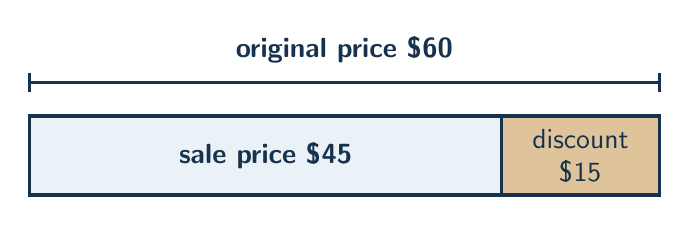
\begin{tikzpicture}[x=1cm,y=1cm]
  % Bar: 8 units total, split at 6 (45 of 60 dollars)
  \fill[qraPale] (0,0) rectangle (6,1);
  \fill[qraGold!45] (6,0) rectangle (8,1);
  \draw[qra axis] (0,0) rectangle (8,1);
  \draw[qra axis] (6,0) -- (6,1);
  \node[qra label] at (3,0.5) {sale price \$45};
  \node[qra small label, align=center] at (7,0.5) {discount\\\$15};
  % Bracket spanning the whole bar
  \draw[qra tick] (0,1.3) -- (0,1.55);
  \draw[qra tick] (8,1.3) -- (8,1.55);
  \draw[qra tick] (0,1.425) -- (8,1.425);
  \node[qra label, above] at (4,1.55) {original price \$60};
\end{tikzpicture}
\end{document}
